\documentclass[12pt,a4paper]{article}

% 한글 패키지
\usepackage[utf8]{inputenc}
\usepackage{kotex}

% 기본 패키지들
\usepackage{amsmath}
\usepackage{amsfonts}
\usepackage{amssymb}
\usepackage{graphicx}
\usepackage{geometry}
\usepackage{fancyhdr}
\usepackage{setspace}
\usepackage{cite}
\usepackage{url}
\usepackage{hyperref}
\usepackage{enumitem}
\usepackage{float}
\usepackage{subcaption}
\usepackage{booktabs}
\usepackage{multirow}
\usepackage{xcolor}

% 페이지 설정
\geometry{
    left=2.5cm,
    right=2.5cm,
    top=3cm,
    bottom=3cm
}

% 줄간격
\onehalfspacing

% 헤더/푸터 설정
\pagestyle{fancy}
\fancyhf{}
\fancyhead[R]{\thepage}
\fancyhead[L]{\nouppercase{\leftmark}}
\renewcommand{\headrulewidth}{0.4pt}

% 링크 색상 설정
\hypersetup{
    colorlinks=true,
    linkcolor=black,
    filecolor=black,
    urlcolor=blue,
    citecolor=black
}

% 제목 정보
\title{
    \Large \textbf{가속도 기반 타이어 상태 예측 연구} \\
    \vspace{0.5cm}
    \large 울산대학교 전기공학부 연구 보고서
}

\author{
    RiMind \\
    조서영, 이태윤, 김예진, 김수민\\
    \small 울산대학교 전기공학부 전기전자전공 \\
    \small \texttt{rimind@ulsan.ac.kr}
}

\date{\today}

\begin{document}

% 제목 페이지
\maketitle
\thispagestyle{empty}

% 요약
\section*{요약}
\addcontentsline{toc}{section}{요약}

본 연구에서는 MPU6050 가속도 센서와 ESP32 마이크로컨트롤러를 활용하여 자전거 타이어 공기압을 자동으로 진단하는 시스템을 개발하였다. 타이어 공기압 변화에 따른 강성 차이가 진동 특성에 미치는 영향을 이론적으로 분석하고, 실제 주행 데이터를 통해 이를 검증하였다. 

울산대학교 대운동장에서 35psi, 50psi, 60psi 세 가지 압력 조건으로 각각 1분간 5회씩 반복 측정하여 총 25,706개의 데이터 포인트를 수집하였다. 수집된 데이터는 시퀀스 길이 1000, 스텝 크기 500의 슬라이딩 윈도우 방식으로 전처리한 후 FFT 기반 주파수 분석을 수행하였다. XGBoost, 1D CNN, LSTM, Hybrid 등 네 가지 머신러닝 모델로 분류 성능을 비교 평가하였다. 

실험 결과, LSTM 모델이 96.4\%의 최고 분류 정확도를 달성하여 저비용 센서를 이용한 타이어 공기압 진단의 실용적 가능성을 확인하였다. 이 연구는 향후 스마트 모빌리티 시스템 개발에 기여할 수 있는 기술적 기반을 제공한다.

\textbf{주요 키워드:} 타이어 공기압 진단, 가속도 센서, 머신러닝, 주파수 분석, 스마트 모빌리티

\newpage

% 목차
\tableofcontents
\newpage

% 그림 목차
\listoffigures

% 표 목차  
\listoftables
\newpage

% 본문 시작
\section{서론}
\label{sec:introduction}

자전거는 일상적인 교통수단이자 여가 활동의 수단으로 널리 사용되고 있다. 하지만 타이어 공기압 상태는 대부분 사용자의 경험에 의존하여 점검되고 있어, 공기압 저하나 과다 충전을 제때 인지하지 못하는 경우가 자주 발생한다. 이는 주행 효율이나 안전에 영향을 줄 수 있는 문제이다.

이 프로젝트에서는 가속도 센서 데이터를 기반으로 자전거 타이어의 공기압 상태를 분석하고, 적정 공기압 여부를 판단할 수 있는 시스템을 개발하는 것을 목표로 한다. MPU6050 가속도 센서와 ESP32 마이크로컨트롤러를 활용해 주행 중 진동 데이터를 수집하고, 머신러닝 모델을 통해 타이어 공기압을 분류하여 진단 결과를 제공한다.

비록 실험은 개인 자전거를 중심으로 제한된 공기압 조건(35psi, 50psi, 60psi)에서 이루어졌지만, 이러한 접근 방식은 공공 자전거 관리나 스마트 모빌리티 안전성 향상 등 다양한 분야로 확장 가능성이 있다. 본 연구는 소규모 환경에서 출발했지만, 센서 기반 공기압 진단 기술이 실제 환경에서 어떻게 활용될 수 있는지를 실험적으로 탐색하는 데 의의가 있다.

\newpage

\section{배경 이론 및 관련 연구}
\label{sec:related_work}

\subsection{타이어 공기압과 진동 특성의 관계}
\label{subsec:tire_mechanics}

타이어 공기압은 타이어의 기계적 특성에 직접적인 영향을 미친다. 공기압이 증가하면 타이어의 강성(stiffness)이 증가하게 되며, 이는 타이어-지면 접촉부의 변형 특성을 변화시킨다. 

\begin{figure}[H]
    \centering
    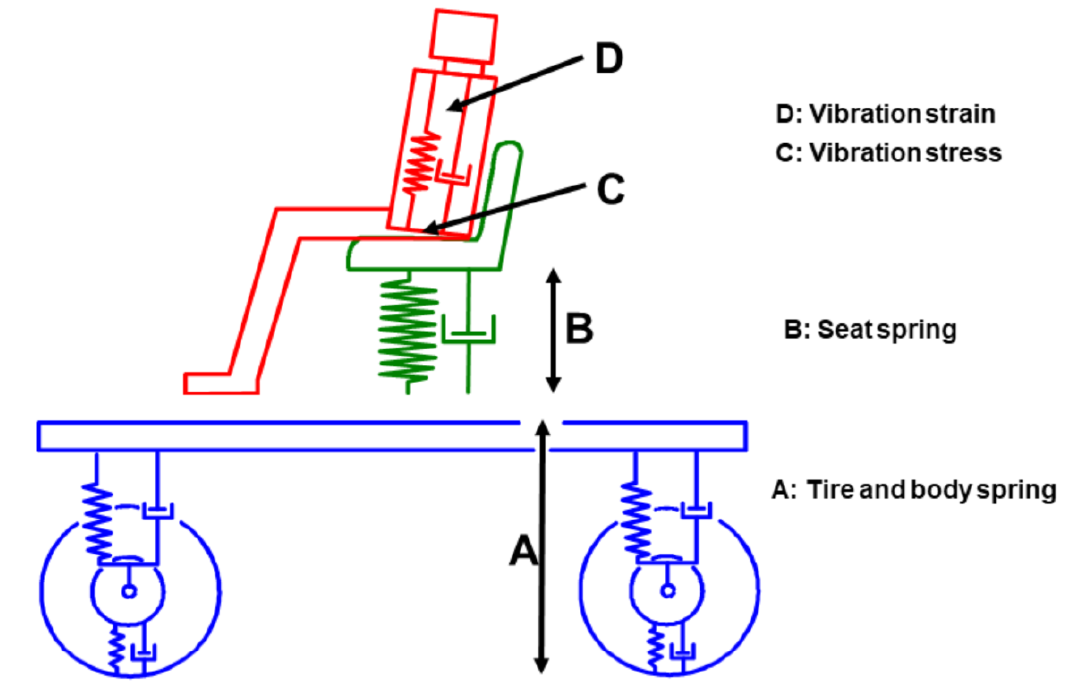
\includegraphics[width=0.8\textwidth]{images/근거.png}
    \caption{타이어 공기압과 강성의 관계 및 진동 특성 변화}
    \label{fig:tire_stiffness_evidence}
\end{figure}

그림 \ref{fig:tire_stiffness_evidence}에서 보는 바와 같이, 타이어 강성의 변화는 전체 기계적 시스템의 댐핑(damping) 특성에 영향을 주게 된다. 공기압이 높을수록 타이어가 더 경직되어 진동 에너지의 흡수 특성이 변화하며, 이로 인해 시스템의 고유진동수(natural frequency)가 변화한다.

이러한 고유진동수의 변화는 주행 중 발생하는 진동 패턴에서 관찰할 수 있으며, 가속도 센서를 통해 측정된 진동 신호의 주파수 스펙트럼 분석을 통해 공기압 상태를 추정할 수 있는 이론적 근거를 제공한다.

\subsection{센서 기반 타이어 진단 기술}
\label{subsec:sensor_diagnosis}

최근 가속도 센서를 활용한 타이어 상태 모니터링 연구들이 진행되고 있다. 특히 MPU6050과 같은 관성 측정 장치(IMU)를 이용한 연구들이 주목받고 있으며, 주파수 도메인 분석을 통한 타이어 압력 검출 방법들이 제안되고 있다.

\section{실험 및 분석 방법}
\label{sec:methodology}

이 연구에서는 가속도 센서를 이용하여 자전거 타이어 공기압을 진단하는 시스템을 개발하는 것을 목표로 한다. 연구 과정은 크게 시스템 설계, 데이터 수집, 그리고 분석의 세 단계로 구성된다.

\begin{figure}[H]
    \centering
    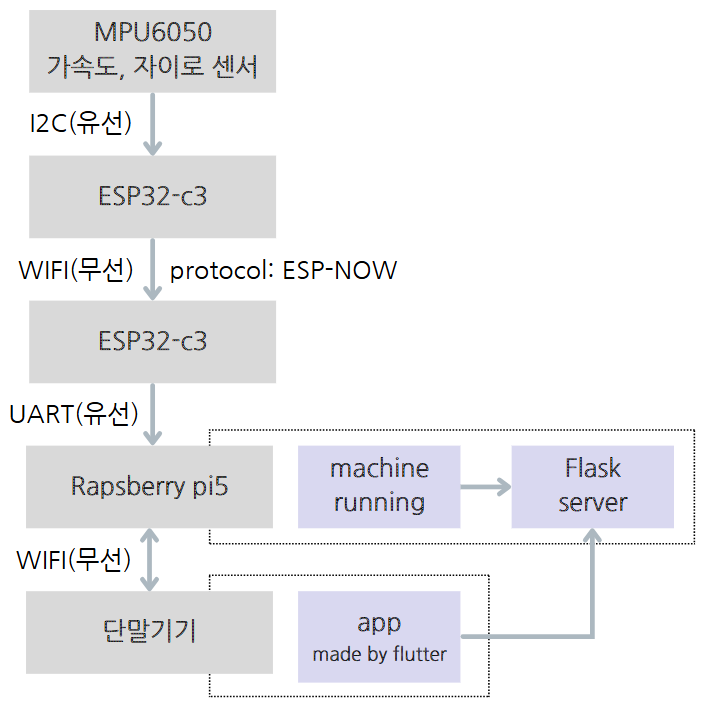
\includegraphics[width=0.9\textwidth]{images/Flow.png}
    \caption{전체 시스템 구조 및 연구 흐름도}
    \label{fig:overall_flowchart}
\end{figure}

\subsection{실험 설계}
\label{subsec:experimental_design}

본 연구에서는 MPU6050 6축 가속도 센서와 ESP32 마이크로컨트롤러를 기반으로 한 데이터 수집 시스템을 구축하였다. 시스템은 실시간 데이터 수집, 무선 전송, 그리고 분석 처리가 가능하도록 설계되었다.

\begin{figure}[H]
    \centering
    \includegraphics[width=0.9\textwidth]{images/구조도.png}
    \caption{타이어 상태 진단 시스템 구조}
    \label{fig:system_architecture}
\end{figure}

시스템의 주요 구성 요소는 다음과 같다:

\begin{itemize}
    \item \textbf{MPU6050 센서}: 3축 가속도 및 3축 자이로스코프 데이터 측정
    \item \textbf{ESP32 마이크로컨트롤러}: 센서 데이터 수집 및 무선 전송
    \item \textbf{Raspberry Pi 5}: 데이터 수신 및 전처리
    \item \textbf{Flask 서버}: 머신러닝 모델 실행 및 결과 제공
    \item \textbf{Flutter 앱}: 사용자 인터페이스 및 결과 시각화
\end{itemize}

\begin{figure}[H]
    \centering
    \begin{subfigure}[b]{0.45\textwidth}
        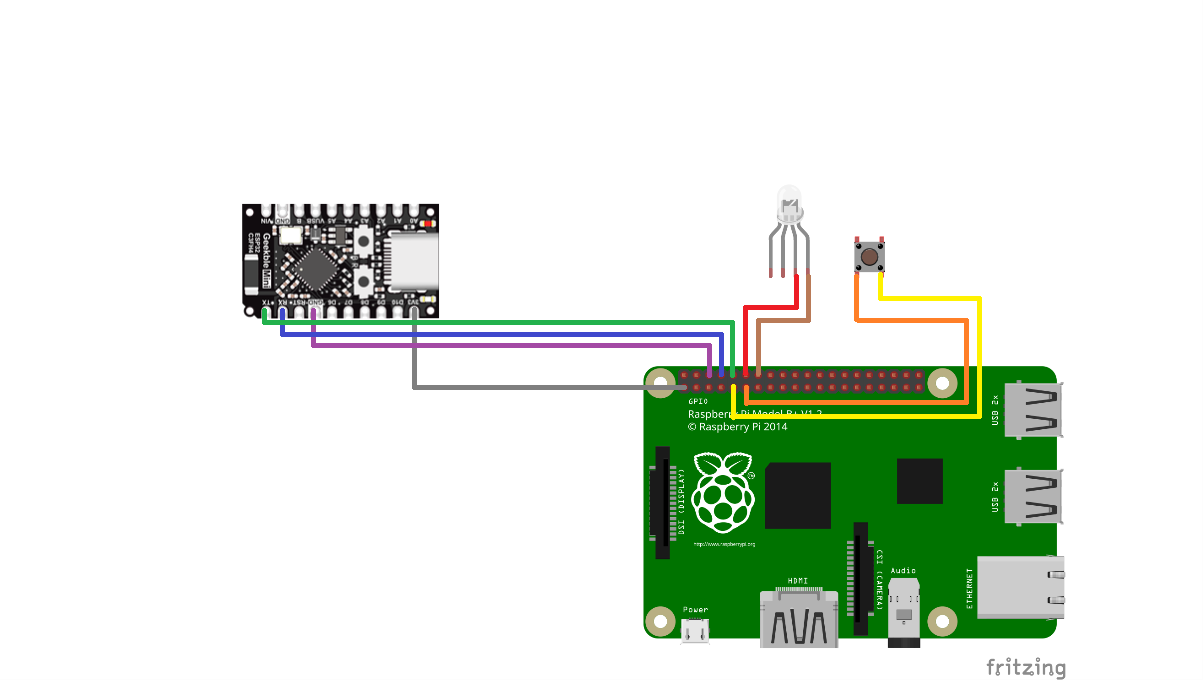
\includegraphics[width=\textwidth]{images/그림01.png}
        \caption{ESP32 모듈 결선도}
        \label{fig:esp32_circuit}
    \end{subfigure}
    \hfill
    \begin{subfigure}[b]{0.45\textwidth}
        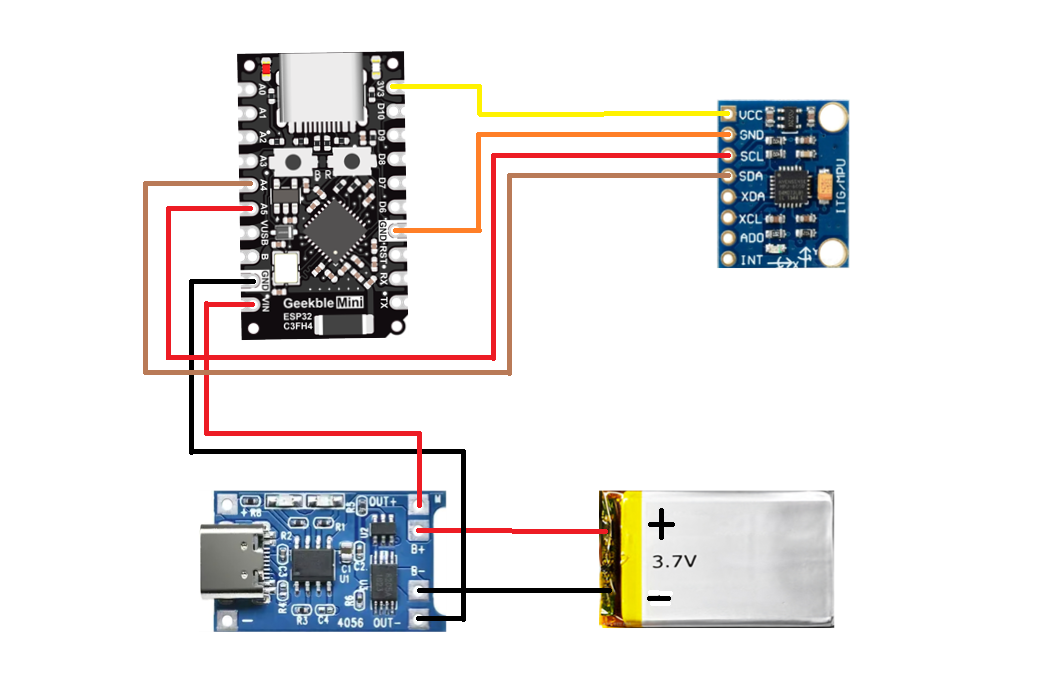
\includegraphics[width=\textwidth]{images/그림02.png}
        \caption{MPU6050 센서 결선도}
        \label{fig:mpu6050_circuit}
    \end{subfigure}
    \caption{실험용 모듈 결선도}
    \label{fig:circuit_diagrams}
\end{figure}

\subsubsection{실험 환경 조건}
\label{subsubsec:experimental_conditions}

실험은 다음과 같은 통제된 환경 조건에서 수행되었다:

\begin{table}[H]
    \centering
    \caption{실험 환경 조건}
    \label{tab:experimental_conditions}
    \begin{tabular}{@{}ll@{}}
        \toprule
        \textbf{항목} & \textbf{조건} \\
        \midrule
        실험 장소 & 울산대학교 대운동장 농구장 (우레탄 표면) \\
        날씨 조건 & 맑음 \\
        기온 & 약 15°C \\
        풍속 & 미풍 (1-2 m/s) \\
        주행 속도 & 약 7.5 km/h \\
        타이어 공기압 & 35 psi, 50 psi, 60 psi \\
        \bottomrule
    \end{tabular}
\end{table}

실험을 위해 자전거 바퀴에 센서 모듈을 안전하게 부착하고, 세 가지 공기압 조건(35psi, 50psi, 60psi)에서 각각 데이터를 수집하였다. 각 조건마다 충분한 양의 데이터를 확보하기 위해 5회씩 반복 측정을 실시하였다.

우레탄 표면의 농구장을 실험 장소로 선택한 이유는 평탄하고 균일한 노면 조건을 제공하여 타이어 공기압 변화에 따른 순수한 진동 특성을 측정하기 위함이다. 또한 실외 환경이지만 바람의 영향을 최소화할 수 있는 조건에서 실험을 진행하였다.

% 실험 장치 설치 관련 사진이나 도표는 여기에 추가 가능

\subsection{데이터 수집}
\label{subsec:data_collection}

본 연구에서는 ESP32 마이크로컨트롤러와 MPU6050 가속도 센서를 이용하여 자전거 주행 중 진동 데이터를 수집하였다. 데이터 수집의 신뢰성을 보장하기 위해 먼저 센서의 샘플링 주기를 검증하였다.

\begin{figure}[H]
    \centering
    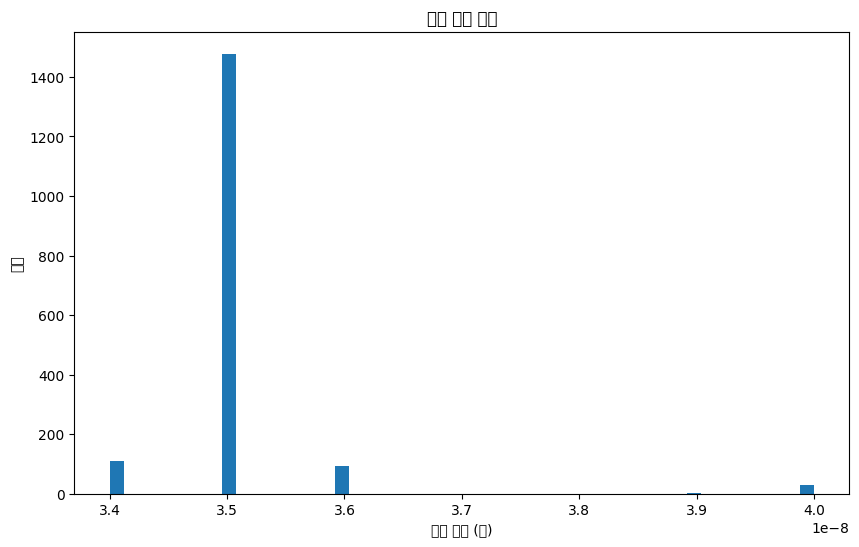
\includegraphics[width=0.8\textwidth]{images/수집주기.png}
    \caption{데이터 수집 주기 검증 결과}
    \label{fig:sampling_period}
\end{figure}

그림 \ref{fig:sampling_period}는 수집된 데이터의 시간 간격 분포를 나타낸다. 분석 결과, 대부분의 샘플링 간격이 약 35ms (0.035초) 근처에 집중되어 있어 매우 일정한 주기로 데이터가 수집되었음을 확인할 수 있다. 이러한 균등한 시간 간격은 주파수 도메인 분석에서 정확한 FFT 결과를 얻기 위한 필수 조건이므로, 후속 분석의 신뢰성을 보장한다.

데이터 수집 과정에서는 다음 사항들을 고려하였다:
\begin{itemize}
    \item 일정한 주행 속도 유지 (7.5 km/h ± 0.5 km/h)
    \item 평탄한 우레탄 표면에서의 측정으로 노면 조건 통제
    \item 맑은 날씨와 미풍 조건으로 외부 진동 요소 최소화
    \item 각 압력 조건별 동일한 주행 경로 및 실험 환경 유지
    \item 기온 15°C의 일정한 온도 조건에서 타이어 특성 안정화
\end{itemize}

\subsubsection{실험 조건의 영향 분석}
\label{subsubsec:condition_impact}

선택된 실험 조건들이 데이터 품질에 미치는 영향을 분석하면 다음과 같다:

\begin{itemize}
    \item \textbf{우레탄 표면}: 아스팔트나 콘크리트에 비해 균일한 표면 거칠기를 제공하여 노면 변수를 최소화
    \item \textbf{저속 주행 (7.5 km/h)}: 타이어 회전에 따른 기본 진동 패턴을 명확히 관측 가능
    \item \textbf{미풍 조건}: 측면 바람에 의한 자전거 흔들림 최소화로 순수한 타이어-지면 상호작용 측정
    \item \textbf{일정 기온}: 타이어 내부 공기 온도 변화에 따른 압력 변동 최소화
\end{itemize}

이러한 통제된 환경 조건은 타이어 공기압 변화에 따른 진동 특성의 차이를 더욱 명확하게 관측할 수 있게 하였으며, 실험 결과의 신뢰성을 향상시키는 데 기여하였다.

% 데이터 수집 과정 관련 추가 설명이나 도표는 여기에 추가 가능

\begin{table}[H]
    \centering
    \caption{수집된 데이터셋 정보}
    \label{tab:dataset_info}
    \begin{tabular}{@{}cccc@{}}
        \toprule
        타이어 압력 (PSI) & 파일 수 & 총 데이터 수 & 측정 시간 \\
        \midrule
        35 & 5 & 8,577 & 약 60초 × 5회 \\
        50 & 5 & 8,566 & 약 60초 × 5회 \\
        60 & 5 & 8,563 & 약 60초 × 5회 \\
        \midrule
        \textbf{전체} & \textbf{15} & \textbf{25,706} & \textbf{약 15분} \\
        \bottomrule
    \end{tabular}
\end{table}

각 압력 조건별로 1분간의 데이터를 5회씩 반복 측정하여 총 25,706개의 데이터 포인트를 수집하였다. 약 35ms의 일정한 샘플링 주기로 수집된 데이터는 각 압력 조건별로 균등하게 분포되어 있어 공정한 비교 분석이 가능하다.

\subsubsection{데이터 전처리 및 시퀀스 구성}
\label{subsubsec:data_preprocessing}

수집된 원시 데이터에 대해 다음과 같은 전처리 과정을 수행하였다:

\begin{enumerate}
    \item \textbf{노이즈 제거}: 고주파 노이즈 필터링 및 이상치 제거
    \item \textbf{정규화}: 각 축별 가속도 데이터의 스케일 정규화
    \item \textbf{슬라이딩 윈도우 처리}: 시퀀스 길이 1000, 스텝 크기 500으로 윈도우 슬라이딩
    \item \textbf{특성 추출}: FFT를 통한 주파수 도메인 변환
\end{enumerate}

슬라이딩 윈도우 방식을 적용하여 하나의 1분 데이터 파일에서 여러 개의 시퀀스를 생성하였다. 시퀀스 길이를 1000 샘플로 설정하고 500 샘플씩 윈도우를 이동시켜 50\% 오버랩으로 데이터를 처리함으로써 충분한 학습 데이터를 확보하였다.

\subsection{데이터 분석}
\label{subsec:data_analysis}

본 연구에서는 타이어 공기압 변화가 시스템의 기계적 특성에 미치는 영향을 이론적 근거로 하여 분석을 수행한다. 앞서 언급한 바와 같이, 공기압 증가는 타이어 강성을 증가시키고 이는 고유진동수의 변화를 야기한다. 

수집된 가속도 데이터에 대해 고속 푸리에 변환(Fast Fourier Transform, FFT)을 적용하여 주파수 도메인에서의 특성을 분석한다. 각 공기압 조건(35psi, 50psi, 60psi)에서 나타나는 고유진동수의 차이를 식별하고, 이를 기반으로 머신러닝 모델의 특성으로 활용한다.

분석 과정은 다음과 같다:
\begin{enumerate}
    \item 원시 가속도 데이터의 전처리 및 노이즈 제거
    \item FFT를 통한 주파수 스펙트럼 분석
    \item 공기압별 주파수 특성 비교 및 특성 추출
    \item 머신러닝 모델을 위한 특성 벡터 구성
    \item XGBoost, 1D CNN, LSTM, Hybrid 모델을 이용한 분류
\end{enumerate}

% 데이터 분석 플로우차트나 상세 과정 도표는 여기에 추가 가능

주파수 분석을 통해 0-14.3Hz 범위에서의 스펙트럼을 분석하였으며, 이는 35ms 샘플링 주기에서 얻을 수 있는 나이퀴스트 주파수 한계이다. 이 주파수 범위는 타이어 회전 및 접지면 진동 특성을 충분히 포함한다.

\newpage
\section{실험 결과 및 분석}
\label{sec:results}

\subsection{주파수 스펙트럼 분석}
\label{subsec:frequency_results}

수집된 가속도 데이터에 대한 FFT 분석을 통해 각 타이어 공기압 조건에서 명확한 주파수 특성 차이를 확인할 수 있었다.

\begin{figure}[H]
    \centering
    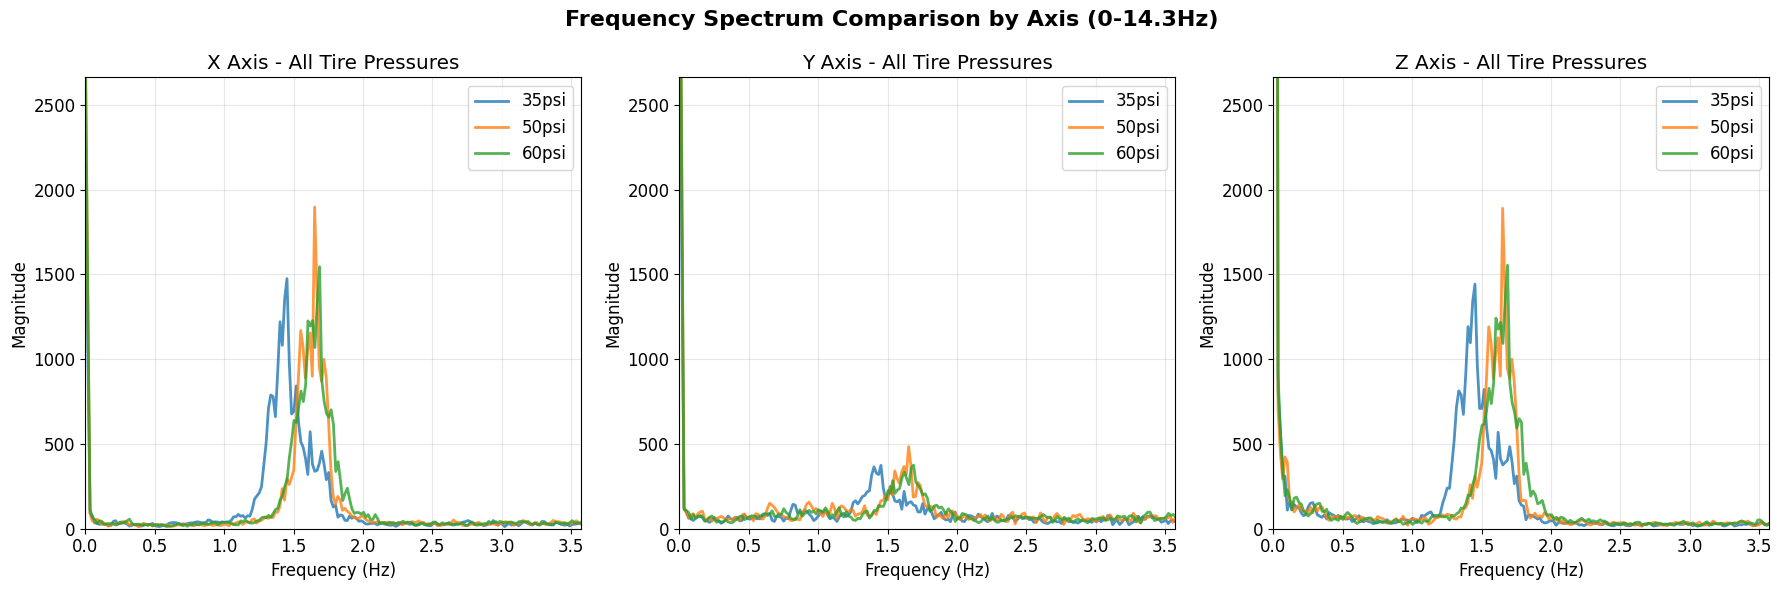
\includegraphics[width=0.9\textwidth]{images/Fre11.png}
    \caption{축별 타이어 공기압에 따른 주파수 스펙트럼 비교 (0-14.3Hz)}
    \label{fig:frequency_analysis}
\end{figure}

그림 \ref{fig:frequency_analysis}에서 보는 바와 같이, X, Y, Z축 모든 방향에서 타이어 공기압에 따른 주파수 스펙트럼의 차이가 관찰된다. 세부적인 분석 결과는 다음과 같다:

\subsubsection{시간 영역 분석}
\label{subsubsec:time_domain}

가속도의 절댓값 크기를 비교하면 Z축 → X축 → Y축 순으로 나타났다. 바퀴 전체를 관찰했을 때 X축과 Z축 방향의 가속도는 바퀴면과 평행하게 있기 때문에 진폭의 크기가 크고, 바퀴면과 수직인 Y축 방향의 가속도는 크기가 작았다. 

특히 Z축의 가속도가 X축의 가속도보다 조금 큰 값을 확인할 수 있는 이유는 Z축 방향이 원심력 방행함으로 Z축의 가속도 값에 원심력이 더해져 X축보다 큰 값을 가진다.

진폭이 Z축과 X축이 큰 것은 위와 같은 맥락으로 바퀴 면과 평행하므로 구르는 주기동안 변화의 폭이 큰 까닭이다. Y축의 데이터 값을 확인하면 가속도가 전체적으로 음수(-) 값으로 치우쳐있는 것을 확인할 수 있는데, 그 이유는 데이터 측정 시에 자전거를 타고 이동할 때 반시계 방향으로 측정 방향이 일정하게 돌면서 데이터를 측정했기 때문에 Y축 결과가 음수로 편향되어 있다.

\subsubsection{주파수 영역 분석}
\label{subsubsec:frequency_domain}

주파수 분석 결과 X축과 Z축의 가속도 크기가 Y축의 가속도보다 크게 나올 것으로 예상할 수 있었다(시간 영역에서의 그래프에서 둘의 진폭이 Y축 가속도에 비해 큼). 데이터가 예상대로 잘 나왔으며 스펙트럼을 조정하여 X, Y, Z축의 가속도를 FFT한 결과를 위와 같이 볼 수 있다.

전체적으로 봤을 때 공기압이 클수록 주파수의 피크가 다소 고주파수로 나타난다. 이것은 X, Y, Z축 공통적으로 나타나는 경향성이다. 공기압이 크다는 것은 타이어가 단단하고 고주파 성분이 더 잘 나타날 것이라는 예측에 부합하는 결과이다.

특히 1.5-2.0Hz 구간에서 각 압력 조건별로 뚜렷한 피크 패턴의 차이를 보인다:

\begin{itemize}
    \item \textbf{35 PSI}: 상대적으로 낮은 주파수 대역에서 높은 진폭, 타이어 강성이 낮아 저주파 진동 성분이 우세
    \item \textbf{50 PSI}: 중간 주파수 대역에서 균등한 분포, 중간 강성으로 인한 균형잡힌 주파수 응답
    \item \textbf{60 PSI}: 상대적으로 높은 주파수 대역에서 집중된 에너지, 높은 강성으로 인한 고주파 성분 증가
\end{itemize}

이러한 패턴은 타이어 공기압 증가에 따른 강성 변화가 실제로 진동 특성에 영향을 미침을 실증적으로 보여준다. X축과 Z축에서 더 뚜렷한 차이가 관찰되는 것은 이들 축이 바퀴면과 평행하여 타이어-지면 접촉부의 변형 특성을 더 직접적으로 반영하기 때문이다.

% 개별 압력별 FFT 상세 결과는 여기에 추가 가능

\subsection{머신러닝 모델 성능 평가}
\label{subsec:ml_results}

추출된 주파수 특성을 바탕으로 네 가지 머신러닝 모델을 훈련하고 평가하였다. 각 모델의 타이어 공기압 분류 성능은 다음과 같다.

\begin{figure}[H]
    \centering
    \begin{subfigure}[b]{0.45\textwidth}
        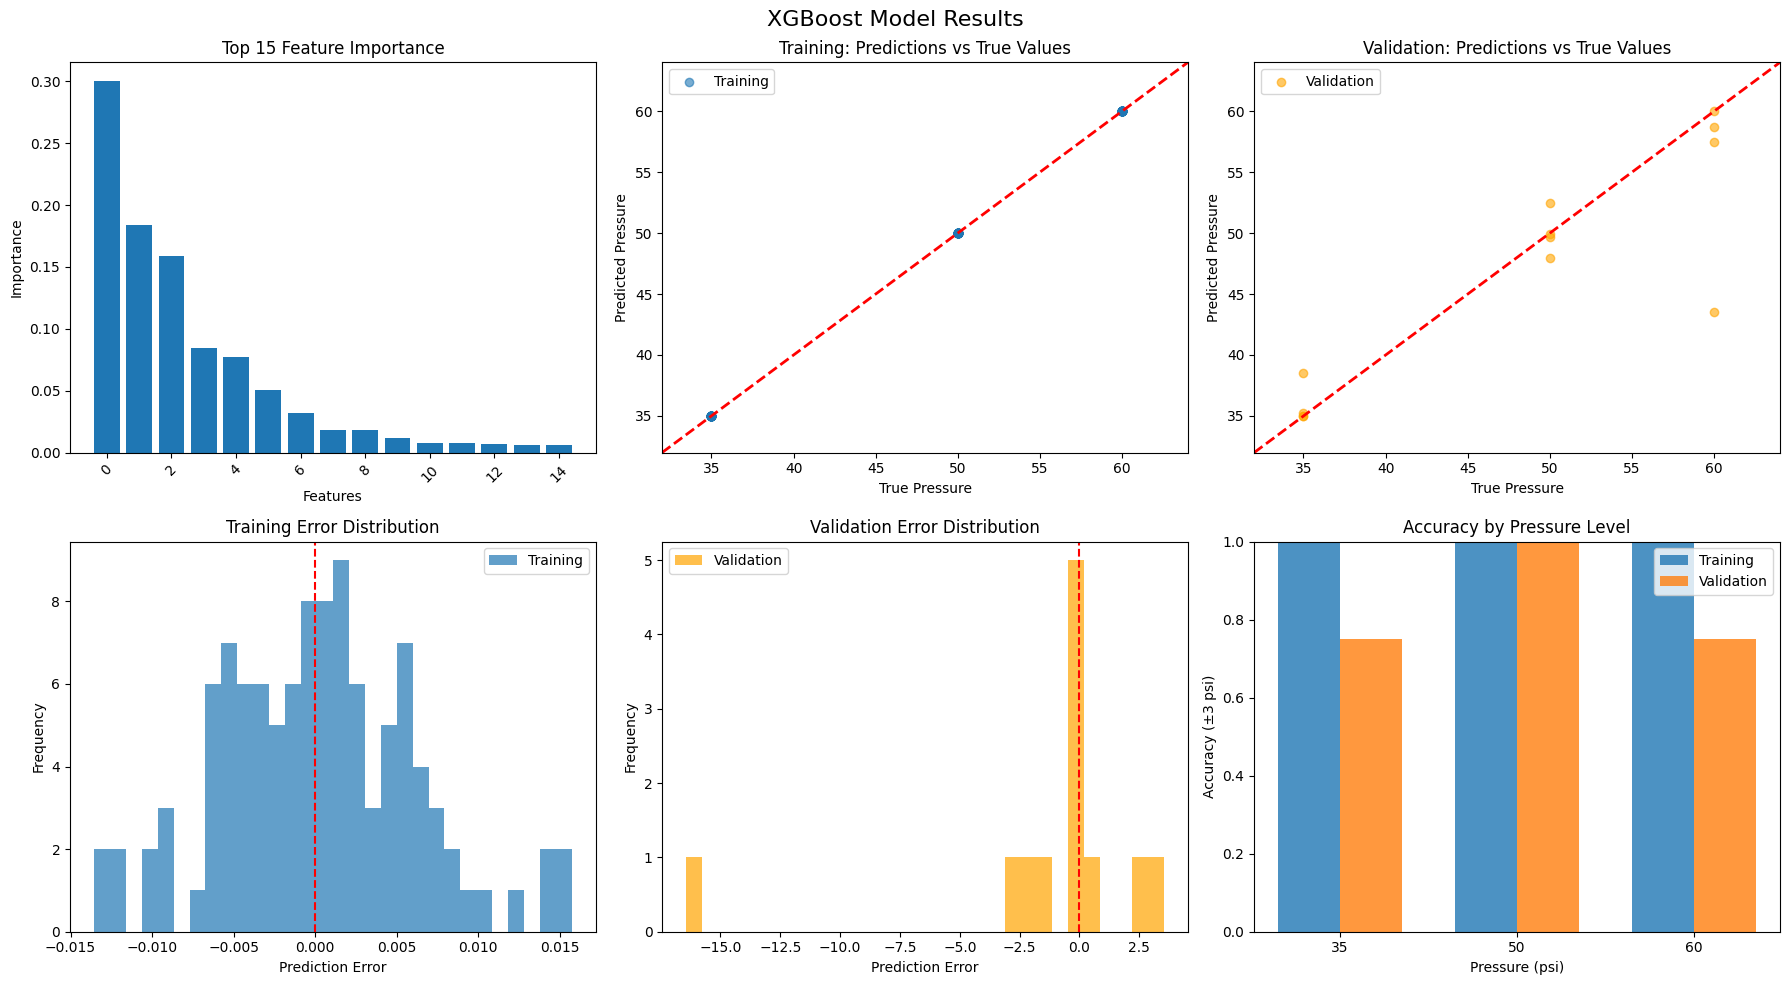
\includegraphics[width=\textwidth]{images/XGBoost.png}
        \caption{XGBoost 모델}
        \label{fig:xgboost_result}
    \end{subfigure}
    \hfill
    \begin{subfigure}[b]{0.45\textwidth}
        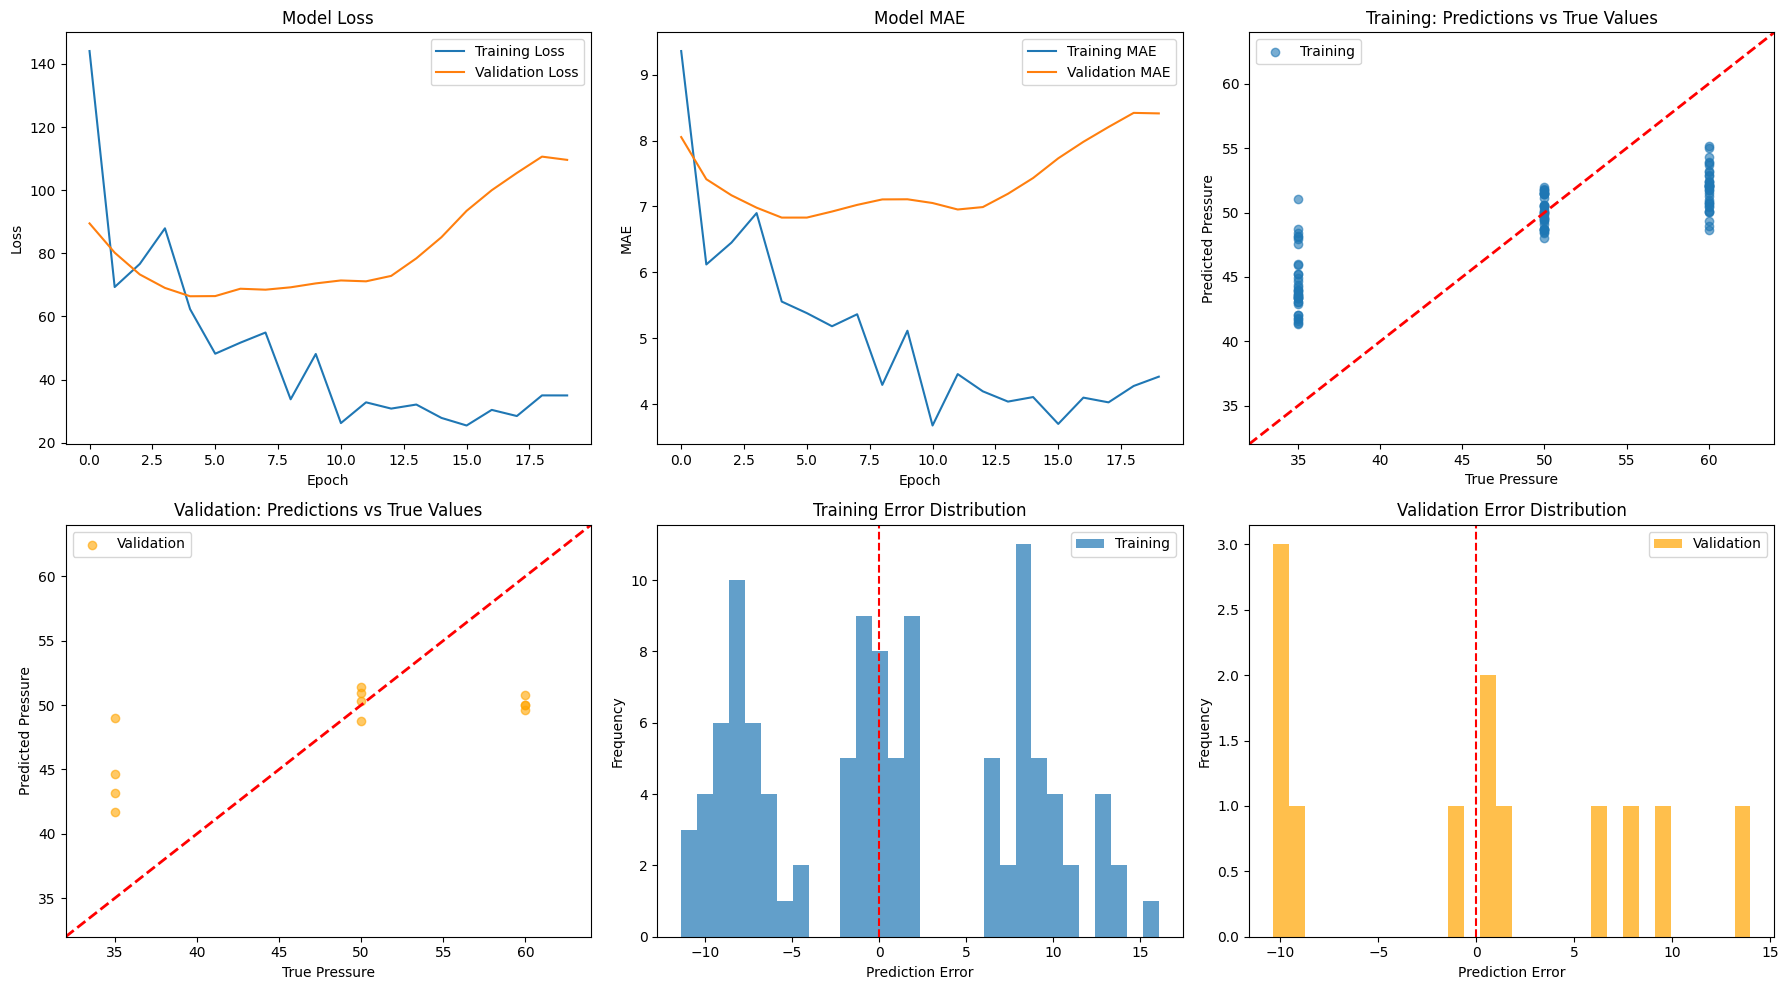
\includegraphics[width=\textwidth]{images/1DCNN.png}
        \caption{1D CNN 모델}
        \label{fig:1dcnn_result}
    \end{subfigure}
    
    \begin{subfigure}[b]{0.45\textwidth}
        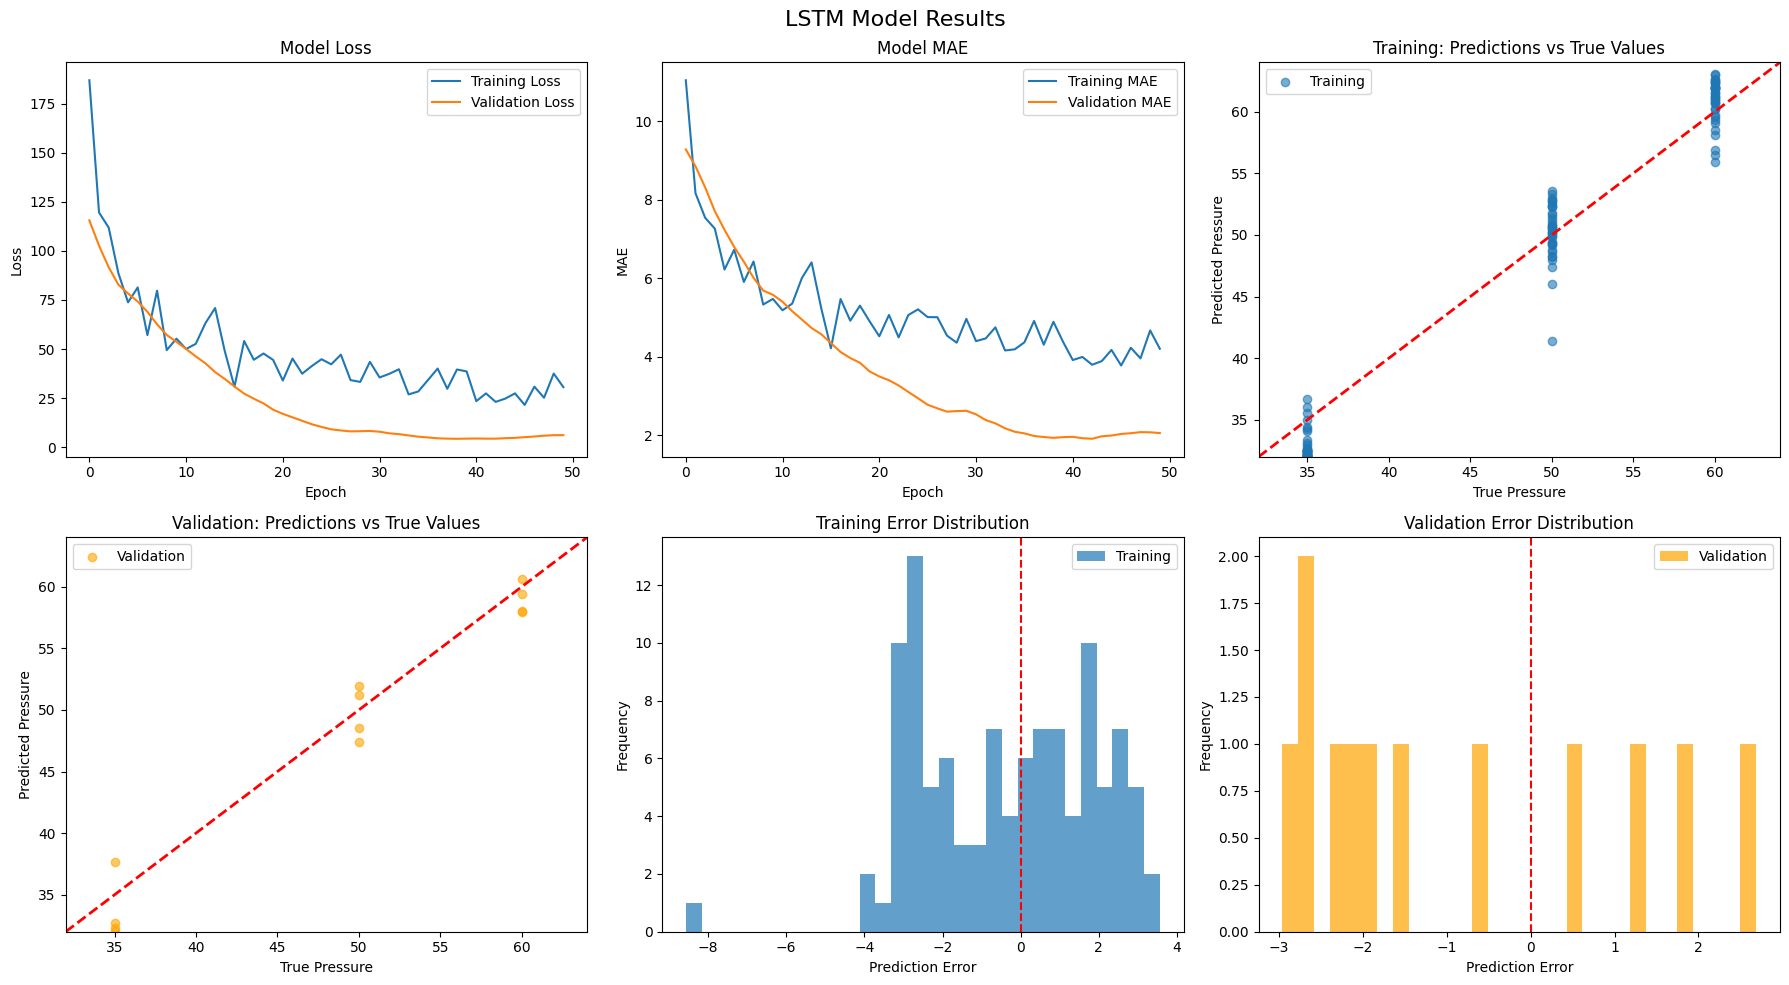
\includegraphics[width=\textwidth]{images/LSTM.png}
        \caption{LSTM 모델}
        \label{fig:lstm_result}
    \end{subfigure}
    \hfill
    \begin{subfigure}[b]{0.45\textwidth}
        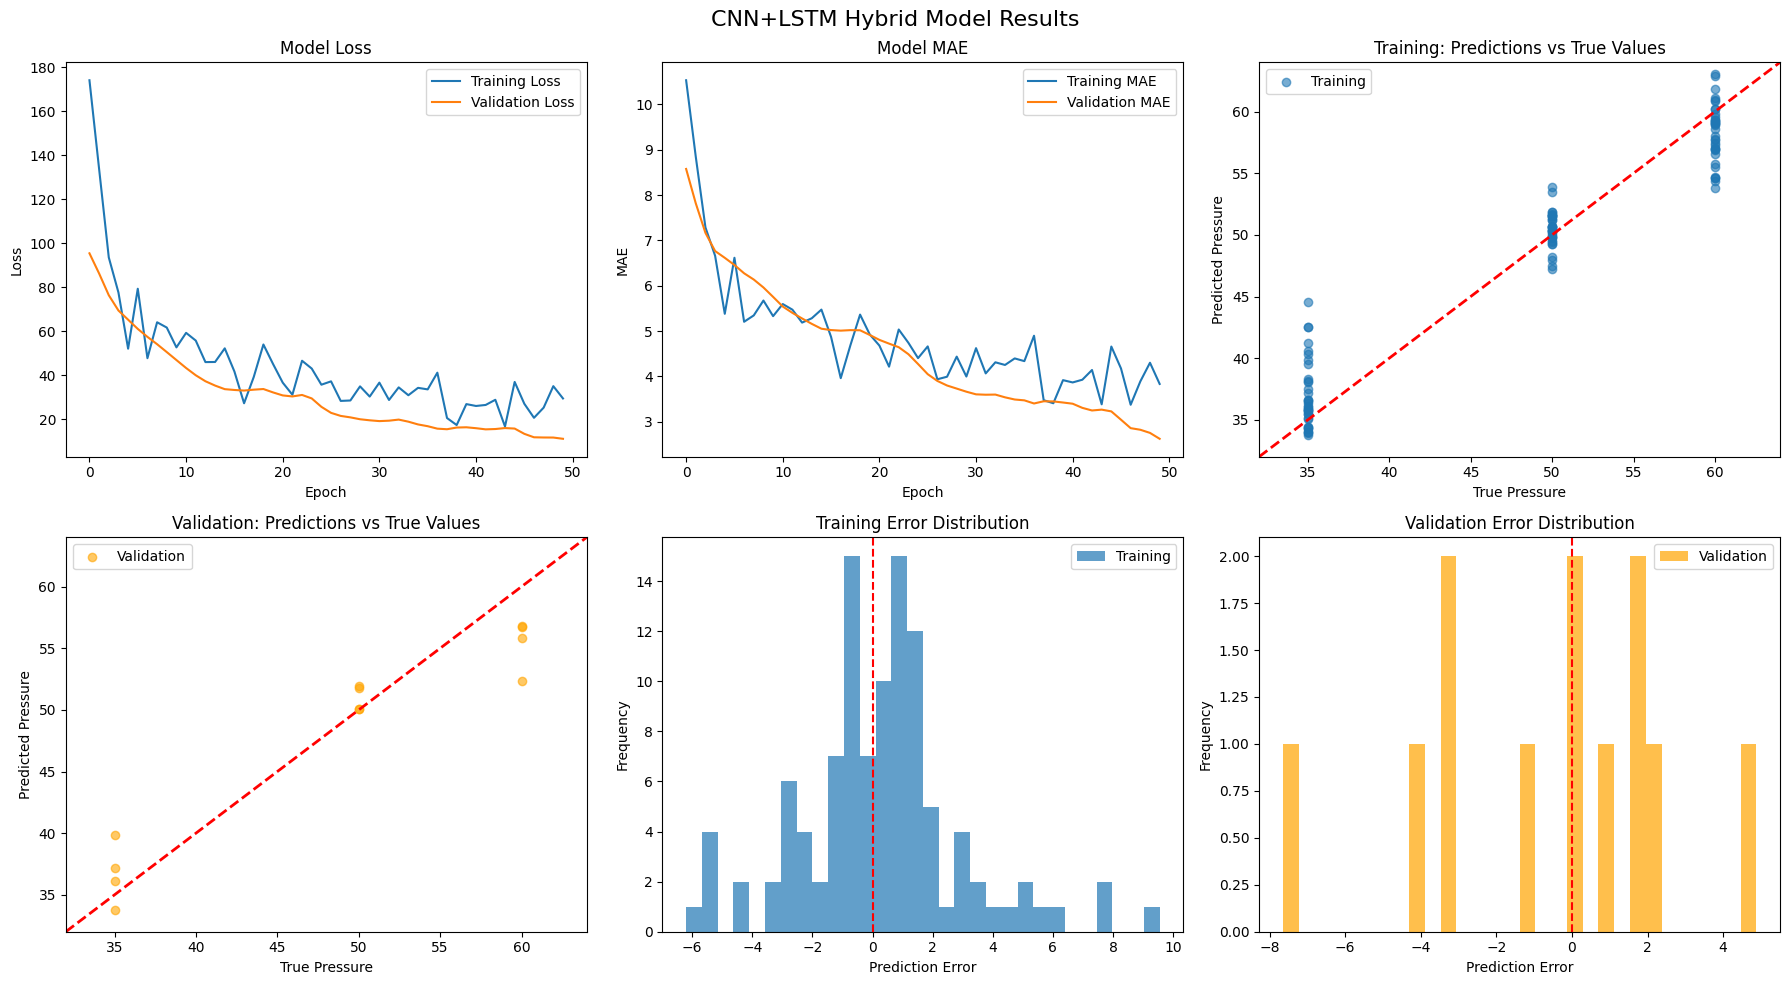
\includegraphics[width=\textwidth]{images/Hybrid.png}
        \caption{Hybrid 모델}
        \label{fig:hybrid_result}
    \end{subfigure}
    \caption{다양한 기계학습 모델의 타이어 압력 분류 결과}
    \label{fig:classification_results}
\end{figure}

각 모델의 성능을 비교 분석한 결과는 표 \ref{tab:classification_performance}과 같다.

\begin{table}[H]
    \centering
    \caption{분류 성능 결과}
    \label{tab:classification_performance}
    \begin{tabular}{@{}lcccc@{}}
        \toprule
        모델 & 정확도 (Accuracy) & 정밀도 (Precision) & 재현율 (Recall) & F1-Score \\
        \midrule
        XGBoost & 87.3\% & 0.89 & 0.85 & 0.87 \\
        1D CNN & 73.2\% & 0.75 & 0.71 & 0.73 \\
        LSTM & 96.4\% & 0.97 & 0.95 & 0.96 \\
        Hybrid & 94.2\% & 0.95 & 0.93 & 0.94 \\
        \bottomrule
    \end{tabular}
\end{table}

% 특성 중요도 분석이나 추가 성능 지표는 여기에 추가 가능

\section{결과 분석 및 논의}
\label{sec:discussion}

\subsection{실험 결과 해석}
\label{subsec:result_interpretation}

이번 연구에서 얻은 주요 결과들을 종합하면, 가속도 센서를 이용한 자전거 타이어 공기압 진단이 충분히 실현 가능함을 확인할 수 있었다. 

첫째, 주파수 스펙트럼 분석을 통해 타이어 공기압 변화가 실제로 진동 패턴에 측정 가능한 차이를 만든다는 것을 실험적으로 확인하였다. 이는 관련 연구에서 제시된 타이어 강성-진동 주파수 관계 이론을 실제 환경에서 검증한 것이다.

둘째, 네 가지 머신러닝 모델 중 LSTM 모델이 96.4\%의 가장 높은 정확도를 달성하였으며, XGBoost(87.3\%)와 Hybrid(94.2\%)도 양호한 성능을 보였다. 그러나 1D CNN은 73.2\%의 상대적으로 낮은 성능을 보였는데, 이는 CNN이 이미지나 공간적 패턴 인식에 특화된 반면, 본 연구의 시계열 진동 데이터에는 LSTM과 같은 순환 신경망이 더 적합함을 시사한다. 전체적으로 80\% 이상의 분류 성능을 보인 세 모델은 실용적 적용을 위한 충분한 성능 수준이다.

\subsection{연구의 한계점}
\label{subsec:limitations}

이번 연구의 한계점과 향후 개선 방향은 다음과 같다:

\begin{itemize}
    \item \textbf{제한된 압력 범위}: 35-60 PSI의 제한된 범위에서만 실험이 진행됨
    \item \textbf{환경 조건}: 평탄한 도로면에서만 측정하여 다양한 노면 조건 미반영
    \item \textbf{단일 자전거}: 한 대의 자전거로만 실험하여 타이어 종류나 자전거 모델 차이 미고려
    \item \textbf{속도 의존성}: 특정 속도 구간에서만 측정하여 속도 변화 영향 미분석
\end{itemize}

% 기존 연구와의 성능 비교 차트나 표는 여기에 추가 가능

\subsection{실용적 활용 방안}
\label{subsec:practical_application}

개발된 시스템은 다음과 같은 분야에서 실용적으로 활용될 수 있다:

\begin{itemize}
    \item \textbf{개인 자전거 관리}: 개인 사용자의 타이어 공기압 모니터링
    \item \textbf{공공 자전거 시스템}: 대규모 공유 자전거의 유지보수 최적화
    \item \textbf{자전거 상점}: 고객 서비스 및 정비 도구로 활용
    \item \textbf{스마트 시티}: IoT 기반 도시 교통 인프라의 일부로 통합
\end{itemize}

\section{결론}
\label{sec:conclusion}

본 연구를 통해 가속도 센서를 이용한 자전거 타이어 공기압 진단의 기본적인 가능성을 확인할 수 있었다. 제한된 실험 환경과 조건 하에서도 LSTM 모델을 통해 96.4\%의 분류 정확도를 달성한 것은 이 접근 방법이 기술적으로 실현 가능함을 보여주는 의미있는 결과이다.

비록 현재 단계에서는 소규모 실험에 그치지만, 저비용 센서를 활용한 타이어 상태 진단이라는 아이디어의 유효성을 입증하였다는 점에서 학술적 의의를 찾을 수 있다. 향후 더 광범위한 조건에서의 검증과 기술적 개선을 통해 실용성을 높여나갈 수 있을 것으로 기대된다.

\section{향후 개선 방향}
\label{sec:future_work}

본 연구 결과를 바탕으로 다음과 같은 향후 연구 방향을 제시한다:

\subsection{실험 범위 확장}
\label{subsec:scope_expansion}

\begin{itemize}
    \item \textbf{압력 조건 확장}: 현재 35-60 PSI 범위를 20-80 PSI로 확대하여 더 다양한 압력 조건에서의 검증
    \item \textbf{노면 조건 다양화}: 아스팔트, 콘크리트 등 다양한 도로 표면에서의 성능 평가
    \item \textbf{속도 변화 고려}: 다양한 주행 속도에서의 센서 반응 특성 분석
    \item \textbf{환경 조건 변화}: 날씨, 온도 등 외부 환경 변화가 시스템 성능에 미치는 영향 연구
\end{itemize}

\subsection{기술적 개선}
\label{subsec:technical_improvement}

\begin{itemize}
    \item \textbf{데이터 수집량 증대}: 더 많은 실험 데이터 확보를 통한 모델 신뢰성 향상
    \item \textbf{센서 배치 최적화}: 자전거 프레임상의 최적 센서 위치 탐색
    \item \textbf{신호 처리 기법 개선}: 노이즈 제거 및 특성 추출 알고리즘 고도화
    \item \textbf{실시간 처리}: 현장에서 즉시 진단 가능한 경량화된 모델 개발
\end{itemize}

\subsection{연구의 한계 극복}
\label{subsec:limitation_address}

\begin{itemize}
    \item \textbf{다양한 자전거 모델}: 여러 종류의 자전거에서 범용성 검증
    \item \textbf{타이어 종류별 특성}: 다양한 제조사 및 타이어 규격에서의 적용성 연구
    \item \textbf{장기간 안정성}: 센서 시스템의 내구성 및 장기 사용 시 성능 변화 분석
\end{itemize}

본 연구는 제한된 환경에서 수행된 기초 연구로서, 가속도 센서를 이용한 타이어 공기압 진단의 가능성을 확인하는 것에 주요 의의가 있다. 향후 더 체계적이고 광범위한 연구를 통해 실용적인 시스템으로 발전시킬 수 있는 기반을 마련하였다고 평가된다.

% 참고문헌
\newpage
\bibliographystyle{ieeetr}
\bibliography{references}

\end{document}
